\documentclass{article}
\usepackage{graphicx}
\graphicspath{ {./} }

\title{Graph based relation learning with SUBDUE}
\author{Samuel Wehunt}
\date{\today}

\begin{document}
\maketitle

\section{}
The output is provided in the file question1Out.txt.\\
the best substructure is as follows:

\texttt{
\\
v 1 object\\
v 2 object\\
v 3 triangle\\
v 4 square\\
d 1 3 shape\\
d 2 4 shape\\
d 1 2 on\\
}

Basically it is saying that the best substructure is composed of 2 objects
the first object is a square, the second is a triangle, and the first object 
is on top of the second object. this makes sense because if we look at the 
picture of the sample in the users handbook then we see this substructure
repeated multiple times.

\section{}
input file is provided as question2In.g\\
output file is provided as question2Out.txt

\section{}
input file is provided as question3In.g\\
output file is provided as question3Out.txt

\section{}
Working with subdue for the benzene rings was pretty interesting; I initially
had hoped for a more interesting output when it analysed the ring examples,
but with the simple structure of the benzene rings I am not surprised at the
rather boring output of the analysis. subdue essentially provided output
that was identical to the input I gave it. The main difference I noticed 
between questions 2 \& 3 was the scores it gave each substructure. in the
analysis without the negative examples, it scored all of the substructures
almost equally, with the correct one just barely winning out. However, when
negative examples were introduced it gave the incorrect substructures a much
lower score than the correct example, which shows me that it had a much better
'understanding' of what a benzene ring is or isn't.\\
I've also noticed that subdue is relatively optimized. the small tests took .01
seconds or less, and when I scaled the input to a file with over 1200 lines, it
only took around .08 seconds, which seems very good.

\section{}
I used a python script to convert the file format to what I needed; it is called
atom\_bond\_translate.py. \\
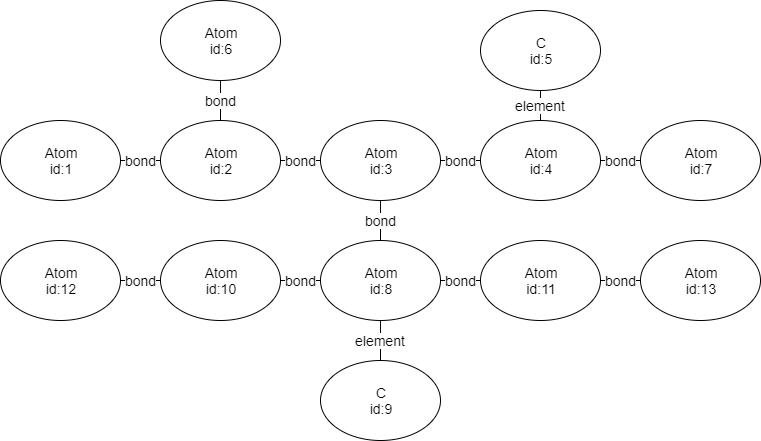
\includegraphics[scale=.5]{question5Pic.png}
This is a drawing of the output from SUBDUE. This structure can be described as
2 chains of atoms connected by one bond. each chain has 5 atoms in it (with
one chain having an atom hanging off). most of the atoms are generic (no
element associated with it), but 2 of them are carbon atoms.
The subdue output is in question5Out.txt.

\section{}
The same script was modified to add the extra vertices and edges which contain 
information about charges and bond types, the updated version can be found in 
atom\_bond\_translate2.py. The file came out to be about 3x the size of the 
previous one.\\
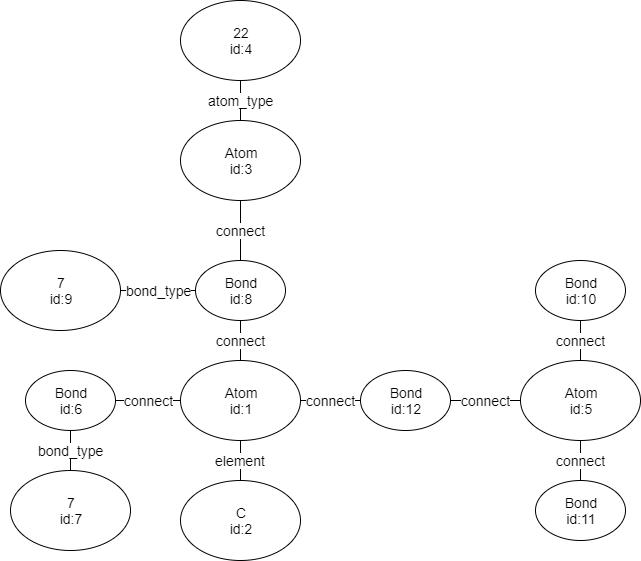
\includegraphics[scale=.5]{question6Pic.png}\\
This drawing is pretty interesting to me because there are far fewer atoms in
it. this tells me that this compound is more specific, and that it is 
potentially better than the previous result. the fact that it took way less
time to compute this result also makes sense, because it implies that SUBDUE
was able to quickly 'dial in' on the patterns related to active compounds.
I don't know chemistry, but it seems like it was able to find a decent indicator
of an 'active' compound.

\section{}
I really enjoyed working with this dataset because for some reason I really like
text processing and manipulating file formats. This problem allowed me to do 
that with some large datasets, and I enjoyed that part. I also found it very
interesting that subdue was able to process the second data file much faster
than the first; despite the fact that the second datafile is about 3 times the
size of the first. To me that indicates that the first file did not contain any
clear indication of what an 'active' compound is, and so it had to do more work
to find out what the best substructure is. Another factor that may affect speed
is the fact that the best substructure for the second dataset is much smaller,
so maybe it did not have to work as hard to match that substructure.

\end{document}
